%%
%% Computer Networks submission — CAS single-column template
%% Compiler: pdfLaTeX (TeX Live 2024)
%% All figures must be in the SAME directory as this .tex file (no subfolders).
%%

\documentclass[a4paper,fleqn]{cas-sc}

\usepackage[numbers,sort&compress]{natbib}

%% Tables
\usepackage{booktabs}
\usepackage{array}
\usepackage{tabularx}
\usepackage{multirow}
\usepackage{makecell}
\usepackage{threeparttable}

%% Math
\usepackage{amsmath}
\usepackage{amssymb}

%% Figures
\usepackage{subcaption}
\usepackage{flafter}
\usepackage{placeins}

%% TikZ (PRISMA flowchart)
\usepackage{tikz}
\usetikzlibrary{shapes.geometric,arrows.meta,positioning,calc}

\usepackage{url}
\usepackage{ragged2e}

%% Allow flexible line-breaking in table p{} columns (prevents overfull hbox)
\renewcommand{\tabularxcolumn}[1]{>{\RaggedRight\arraybackslash}p{#1}}
%% Give LaTeX extra stretch budget for hard-to-break lines
\setlength{\emergencystretch}{3em}

% ============================================================
\begin{document}
\let\WriteBookmarks\relax

% Suppress the CAS template's empty "ORCID(s):" footnote until real ORCID IDs are provided.
\ExplSyntaxOn
\RenewDocumentCommand \printorcid { }
  {
    \seq_if_empty:NF \g_stm_orcid_seq
      {
        \group_begin:
          \tex_let:D \thefootnote \relax \footnotetext
          {
            \raggedright
            \textsc{orcid}(s):\c_space_token
            \seq_use:Nn \g_stm_orcid_seq { ;~ }
          }
        \group_end:
      }
  }
\ExplSyntaxOff

%% Float placement parameters — keep figures near their citations
\setcounter{topnumber}{4}
\setcounter{bottomnumber}{2}
\setcounter{totalnumber}{6}
\renewcommand{\topfraction}{0.85}
\renewcommand{\bottomfraction}{0.5}
\renewcommand{\textfraction}{0.10}
\renewcommand{\floatpagefraction}{0.70}

\shorttitle{BBR Congestion Control: Applicability Boundaries and Fairness}
\shortauthors{Xu et~al.}

\title[mode=title]{Applicability Boundaries and Fairness Challenges of BBR
  Congestion Control: A Three-Dimensional Framework, Version Evolution,
  and Multi-Scenario Evaluation}

\author[1]{Shouzheng Xu}\cormark[1]\fnmark[1]
\credit{Conceptualization, Supervision, Project administration, Writing -- review \& editing}

\author[1]{Ruohan Ma}\fnmark[1]
\credit{Investigation, Writing -- original draft}

\author[1]{Zonglin Feng}\fnmark[1]
\credit{Investigation, Writing -- original draft}

\author[1]{Xinyue Liu}\fnmark[1]
\credit{Investigation, Writing -- original draft}

\author[1]{Tingjia Liu}\fnmark[1]
\credit{Investigation, Writing -- original draft}

\affiliation[1]{organization={School of Information, Central University of
    Finance and Economics},
  city={Beijing}, postcode={100081}, country={China}}

\cortext[1]{Corresponding author. E-mail: xu.shouzheng@email.cufe.edu.cn}
\fntext[1]{All authors contributed equally to this work.}

% ---------- Abstract ----------
\begin{abstract}
Loss-driven congestion control algorithms trade excessive queuing delay for
bandwidth utilization in high bandwidth-delay product (BDP)
networks---a fundamental tension that motivated Google to propose BBR in
2016, followed by BBRv2 (2019) and BBRv3 (2023). Despite three
iterations, a unified framework for BBR's applicability boundaries,
cross-version performance, and fairness mechanisms remains absent.
We conduct a systematic review of 165 peer-reviewed papers, RFC standards,
and technical documents retrieved from IEEE Xplore, ACM DL, Google Scholar,
CNKI, and arXiv (1979--2026), with 60 items from 2023--2026, classified
by evidence quality. We propose a three-dimensional applicability framework
(buffer depth $\times$ BDP magnitude $\times$ loss source) and synthesize
evidence across six representative scenarios: high-BDP WAN, shallow-buffer
wired, broadband multi-flow, high-loss wireless, high-dynamic routing, and
LEO satellite. Key findings: in Google B4 backbone deployments, BBR achieves
median throughput $\approx\!5\times$ CUBIC; in controlled wired testbeds,
BBRv3 improves throughput by $\approx\!48\%$ over CUBIC; however, BBR may
underperform CUBIC in WiFi frame-aggregation and deep-buffer environments.
Intra-protocol RTT unfairness is associated with the interaction between
per-flow path estimates, probing dynamics, and shared-queue conditions;
inter-protocol unfairness stems from fundamentally different loss responses.
Reported multi-RTT simulations show that BBRv3 fairness varies substantially
with buffer and RTT conditions, suggesting that parameter-level revisions alone
may be insufficient to resolve measurement-model limitations.
AI-assisted approaches show promise in controlled settings but face
interpretability, Sim-to-Real transfer, and inference-overhead gaps.
We identify four open research directions: interpretable measurement
modeling, cross-algorithm fairness mechanisms, heterogeneous network
robustness, and deployable AI-assisted congestion control.
\end{abstract}

\begin{highlights}
\item Three-dimensional BBR applicability framework: buffer depth $\times$ BDP $\times$ loss source.
\item 165-reference systematic review covering BBRv1--v3, wireless, and LEO scenarios.
\item BBRv3 fairness remains configuration-dependent across buffer and RTT conditions.
\item Structured six-scenario evaluation with quantified throughput and fairness metrics.
\item Four open problems: modeling, fairness, robustness, and deployable AI.
\end{highlights}

\begin{keywords}
BBR congestion control \sep fairness \sep high-BDP networks \sep
wireless adaptation \sep LEO satellite \sep AI-assisted control \sep applicability boundary
\end{keywords}

\maketitle

% ============================================================
\section{Introduction}
\label{sec:intro}
% ============================================================

\subsection{Background and Motivation}
\label{sec:background}

Building on Jacobson's congestion avoidance algorithm~\citep{jacobson1988congestion},
loss-driven congestion control---represented by CUBIC~\citep{ha2008cubic} and
Reno~\citep{fall1996simulation}---has dominated the Internet transport layer for
decades. The fundamental limitation of such schemes is that their steady-state
operating point lies to the right of Kleinrock's optimal power
point~\citep{kleinrock1979power}: buffers are already full and queuing delay
remains persistently high, a cost that is especially pronounced in backbone
networks with high bandwidth-delay products (BDP). The bandwidth ceiling derived
by Mathis et al.
($\mathrm{BW}_{\max}\approx C\cdot\mathrm{MSS}/(\mathrm{RTT}\cdot\sqrt{p})$)~\citep{mathis1997macroscopic}
theoretically quantifies this constraint: under typical intercontinental link loss
rates, CUBIC's achievable bandwidth is limited to far below the link capacity.
To overcome this constraint, Google proposed BBR (Bottleneck Bandwidth and
Round-trip propagation time) in 2016~\citep{cardwell2017bbr}, replacing
loss-signal-driven reactive control with direct measurement of the bottleneck
bandwidth BtlBw and propagation delay RTprop, and demonstrating significant
throughput advantages over CUBIC in large-scale deployments on Google's B4 WAN.
BBR subsequently released BBRv2 in 2019 (introducing ECN support and in-flight
upper-bound constraints)~\citep{cardwell2019bbrv2} and BBRv3 in 2023 (further
tightening Startup exit conditions)~\citep{cardwell2023bbrv3}. Unlike BBRv1,
which has entered the Linux mainline, BBRv2/BBRv3 continue to evolve primarily
through drafts, implementation prototypes, and independent evaluations. Meanwhile,
QUIC/HTTP~3, LEO satellite measurements, and CDN scenario studies have expanded
BBR's influence beyond the traditional TCP
stack~\citep{rfc9000,rfc9002,rfc9114,deutschmann2023starlink,kamel2024starquic}.

Despite continuous iteration, three deep contradictions persist. First, BBR's
performance exhibits strong scenario dependence: its median throughput in
high-BDP WANs can reach approximately five times CUBIC, yet in WiFi
frame-aggregation environments, its throughput falls below CUBIC due to a
fundamental conflict between uniform pacing and 802.11 burst transmission.
Second, two types of fairness problems remain unresolved across three generations:
intra-protocol RTT bias is rooted in the multiplicative structure of
$\mathrm{BDP}=\mathrm{BtlBw}\times\mathrm{RTprop}$---a geometric constraint
determined by physical quantities---while inter-protocol fairness improvements
depend heavily on ECN/L4S explicit congestion signals whose real-world
availability exhibits strong path dependence; BBRv3 has also been reported to
regress in intra-protocol fairness relative to v2 in large-buffer
scenarios~\citep{rfc3168,rfc9330,rfc9331,rfc9332,piotrowska2024}. Third,
AI-assisted improvements, though demonstrating promise in controlled testbeds
or simulation environments, face three substantial challenges: insufficient
interpretability, structural Sim-to-Real gaps, and real-time inference overhead.

The core reason these contradictions cannot be resolved within existing research
frameworks is the absence of an analytical tool that systematically maps network
environment characteristics to BBR's degree of applicability. Existing findings
are scattered across different network conditions and cannot be integrated into
actionable algorithm selection criteria for network operators, nor can the
improvement potential of AI-assisted schemes be evaluated on a unified dimension.
At the same time, BBR's engineering footprint continues to expand: BBRv1 has
entered the Linux mainline and been widely tested; BBRv2/BBRv3 continue to be
evaluated through IETF drafts, open-source implementations, and independent
measurements; QUIC stacks and LEO satellite link research continually expand the
scope of discussion~\citep{cardwell2017bbr,cardwell2019bbrv2,ietf_ccwg_bbr,abrol2026bbr,zeynali2024bbrv3}.
This tension between expanding engineering influence and the absence of an
analytical framework motivates an urgent systematic survey of BBR's performance
boundaries.

\subsection{Related Surveys and Positioning}
\label{sec:related}

Existing work has revealed BBR's advantages and deficiencies from various angles,
but has not yet answered the three questions readers care most about: when BBR
should be deployed, when it should be used with caution, and why three generations
of evolution have not resolved fairness problems. Early independent evaluations
focused primarily on BBRv1's performance in controlled wired scenarios:
\citet{hock2017bbr} revealed RTT bias, \citet{cao2019bbr} identified the random
loss ``cliff effect,'' and \citet{jaeger2019bbr} and \citet{scholz2018deeper}
provided reproducible experimental baselines. Recent BBRv3 research has pushed
the problem toward fairness and deployment boundaries: \citet{piotrowska2024}
reported that v3's intra-protocol fairness regresses relative to v2 in
large-buffer scenarios, \citet{gomez2024bbrv3} provided real-world broadband
baselines, and \citet{zeynali2024bbrv3} and \citet{bless2025insights} further
revealed extreme unfairness and self-induced queuing on public Internet paths and
high-speed links.

The gap in existing research is therefore not ``has anyone measured BBR,'' but
rather the absence of a survey framework that can translate scattered measurement
results into algorithm selection judgments. Existing surveys such as
\citet{al2019survey} are limited by their publication date and do not cover
BBRv2/v3, wireless, or satellite scenarios; \citet{abrol2026bbr}, while
systematically revealing multi-flow QoS defects in 5G/6G controlled experiments,
has not yet unified WiFi frame aggregation, high-dynamic routing, and LEO
satellites within a boundary framework. Table~\ref{tab:survey_compare} compares
the coverage of this paper with existing work: the goal here is not to pile up
more cases, but to compress them into three tools readers can take away---an
applicability boundary coordinate, a fairness root-cause chain, and an
AI deployability tier.

\begin{table}[pos=tbp]
  \caption{Comparison with existing BBR-related surveys and systematic evaluations.}
  \label{tab:survey_compare}
  \footnotesize
  \setlength{\tabcolsep}{3pt}
  \begin{tabularx}{\tblwidth}{@{}p{3.2cm}p{1.4cm}p{1.1cm}p{0.9cm}p{1.0cm}p{1.2cm}p{0.55cm}p{0.55cm}p{0.9cm}p{1.1cm}@{}}
    \toprule
    \textbf{Work} & \textbf{Type} & \textbf{Ver.} & \makecell[l]{\textbf{Sce-}\\\textbf{narios}}
      & \textbf{Fairness} & \makecell[l]{\textbf{Frame-}\\\textbf{work}} & \textbf{AI} & \textbf{Sat.}
      & \makecell[l]{\textbf{Wire-}\\\textbf{less}} & \makecell[l]{\textbf{Meth-}\\\textbf{odol.}} \\
    \midrule
    \citet{hock2017bbr} (2017) & Meas. & v1 & 1 & Partial & None & No & No & No & No \\
    \citet{cao2019bbr} (2019) & Meas. & v1 & 2 & Partial & None & No & No & No & No \\
    \citet{jaeger2019bbr} (2019) & Meas. & v1 & 3 & $\checkmark$ & None & No & No & No & No \\
    \citet{al2019survey} (2019) & Survey & v1 & 2 & Partial & None & No & No & No & No \\
    \citet{piotrowska2024} (2024) & Simul. & v1--v3 & 1 & $\checkmark$ & None & No & No & No & No \\
    \citet{gomez2024bbrv3} (2024) & Meas. & v3 & 1 & $\checkmark$ & None & No & No & No & No \\
    \citet{abrol2026bbr} (2026) & Survey & v1--v3 & 4 & $\checkmark$ & None & No & No & 5G & No \\
    \citet{zeynali2024bbrv3} (2024) & Meas. & v3 & 1 & $\checkmark$ & None & No & No & No & No \\
    \citet{bless2025insights} (2025) & Meas. & v3 & 2 & Partial & None & No & No & No & No \\
    \textbf{This paper} & \textbf{Survey} & \textbf{v1--v3} & \textbf{6}
      & $\checkmark$ & \textbf{3-D} & $\checkmark$ & $\checkmark$ & $\checkmark$ & $\checkmark$ \\
    \bottomrule
  \end{tabularx}
  \begin{tablenotes}
    \small
    \item ``Methodol.'' indicates whether an explicit literature search protocol is described;
    ``5G'' in the Wireless column indicates coverage of 5G scenarios only.
  \end{tablenotes}
\end{table}

\subsection{Systematic Review Methodology}
\label{sec:method}

To ensure reproducibility and evidence reliability, we employ a structured
literature search strategy with systematic quality stratification.

The search covers IEEE Xplore, ACM Digital Library, Google Scholar, CNKI, arXiv,
the USENIX/ACM open paper repository, and the IETF RFC and Internet Draft
repository, spanning 1979 (the year Kleinrock published his optimal power
theory~\citep{kleinrock1979power}) through May 2026. The core query combines
``BBR'' and ``congestion control'' with Boolean logic, cross-expanded with
modifiers including ``fairness,'' ``wireless,'' ``satellite,'' ``WiFi,'' ``LEO,''
``5G,'' ``reinforcement learning,'' ``QUIC,'' ``L4S,'' ``ECN,'' and ``high BDP.''
To avoid reporting search engine hit counts as verifiable sample sizes, we do not
report raw hit numbers; instead, we use the evidence base actually cited in the
body text as the statistical unit: the reference list contains 165 entries, all
genuinely cited in the text; 60 of these are from 2023--2026, and gray literature
is held to fewer than 10 items, used only for version facts, draft evolution, or
supporting background---never as the sole source for a core quantitative claim.
Inclusion criteria: genuinely cited in the text and directly relevant to BBR
applicability boundaries, congestion control fairness, transmission protocol
evolution, or network-side congestion signals. Exclusion criteria: no verifiable
source, retracted, contains only non-reproducible experimental descriptions, or
lacks direct relevance to the six scenario types or mechanism analyses.

For evidence quality stratification, we classify included literature into three
tiers based on source traceability, peer-review rigor, experimental independence,
environment reproducibility, and parameter disclosure completeness. Tier~1:
top-venue papers, RFC standards, and independent measurement studies with complete
parameter disclosure~\citep{jaeger2019bbr,scholz2018deeper,gomez2024bbrv3,rfc9000,rfc9002,rfc9114,rfc9330,rfc9331,rfc9332}.
Tier~2: controlled testbed or simulation
studies~\citep{hock2017bbr,piotrowska2024,cao2019bbr}. Tier~3: preprints,
drafts, theses, or working group
materials~\citep{ma2017fairness,sologon2025thesis,cardwell2019bbrv2,cardwell2023bbrv3,ietf_ccwg_bbr}.
All percentages, multipliers, throughput values, Jain indices, RTT/BDP thresholds,
and deployment status in subsequent sections must correspond to specific papers,
tables, figures, or standard documents; strong claims that cannot be verified are
deleted, softened, or bounded by experimental conditions.

The 165 references are grouped thematically, serving five areas: BBR model
boundary foundations~\citep{postel1981tcp,allman2009rfc5681,paxson2011rfc6298,rfc8312,rfc8257,brakmo1994vegas,floyd1993red,nichols2012codel,pan2013pie,gettys2011bufferbloat,kelly1998rate,padhye1998modeling,appenzeller2004sizing,dhamdhere2006buffer,wischik2005buffers,blanton2002reorder,jaiswal2007oos,paxson1999dynamics,medina2004transport,barakat2000tcp,zhang2001constancy,jain2002bandwidth,prasad2003bandwidth,dukkipati2006fct,tan2006compound,liu2008illinois,grieco2004westwood,handley2003tfrc,kuzmanovic2006tcplp},
data center and programmable scheduling
boundaries~\citep{alizadeh2010dctcp,alizadeh2013pfabric,bai2015pias,mittal2015timely,zhu2015dcqcn,handley2017ndp,cho2017credit,li2019hpcc,kumar2020swift,liu2021onramp,goyal2022bfc,wang2023poseidon,arslan2023bolt,dhamija2024dctcp,zhang2024lossless,wang2024pudica,zhang2024tecc,addanki2024credence,addanki2024reverie,agarwal2024provably,kumar2024chisel,wydrowski2024prequal,agarwal2024harmony,wang2024smuff,zhou2024augur,zhang2024habitus,du2025pred,liu2025pyrrha,chen2025etran,zhao2025whiteboxing,prasopoulos2025sird,ji2025mtp,zeng2025alibaba,chen2025clubheap,sharafzadeh2025scrr,alcoz2025scheduling,gao2024sifter},
BBR version and independent
evaluation~\citep{cardwell2016bbrqueue,kfoury2020bbrv2alpha,song2021bbrv2,scherrer2022modelbased,gomez2023fabric,pan2021bbracw,zhang2021gamma,yang2023pacinggain,ahsan2023bbrn,yang2019adaptivebbr,sarpkaya2025sharing},
QUIC and deployment
scenarios~\citep{langley2017quic,kakhki2017quic,deconinck2017mpquic,trevisan2021http3,rfc8684,raiciu2012mptcp,yuan2024sidekick,winstein2013sprout,zaki2015verus,xie2020pbecc,michel2022starlink,kassem2022starlink,lai2023starlink,khan2023leo,barbosa2023leo,laniewski2024wetlinks,laniewski2024road,izhikevich2023leo,cheng2024grace,meng2024hairpin},
and learning-based congestion control and experimental
platforms~\citep{dong2015pcc,yang2019adaptivebbr,yan2018pantheon,arun2018copa,narayan2018ccp,abbasloo2020orca,meng2020proteus,netravali2015mahimahi,lantz2010mininet,henderson2008ns3,boutaba2018ml}.

\begin{figure}[pos=tbp]
\centering
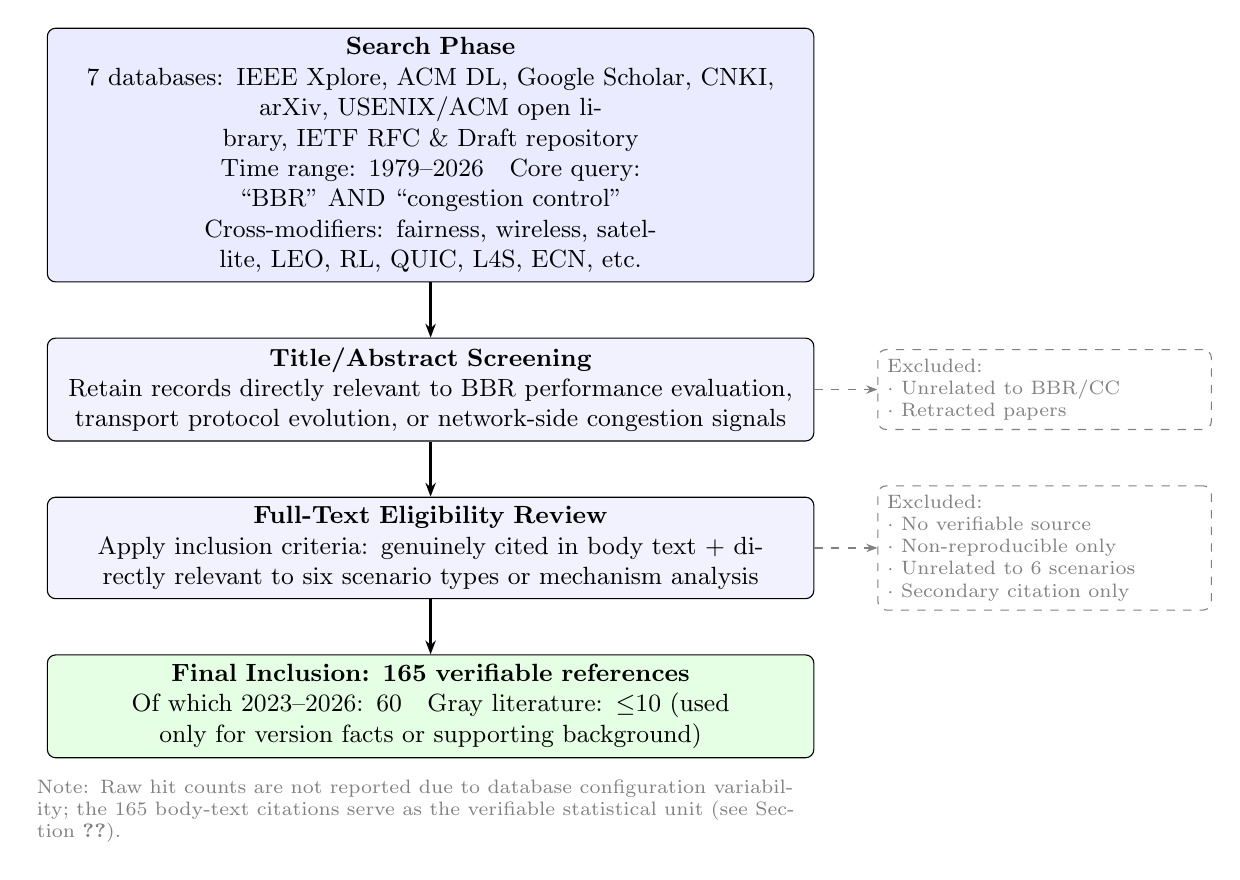
\begin{tikzpicture}[
  node distance=0.7cm,
  box/.style={rectangle, draw=black, rounded corners=3pt,
              text width=9.5cm, align=center,
              minimum height=0.9cm, font=\small},
  excl/.style={rectangle, draw=gray, dashed, rounded corners=3pt,
               text width=4.0cm, align=left,
               minimum height=0.9cm, font=\scriptsize, text=gray},
  arr/.style={-{Stealth[length=5pt]}, thick},
  exclarr/.style={-{Stealth[length=4pt]}, gray, dashed}
]
\node[box, fill=blue!8] (id)
  {\textbf{Search Phase}\\
   7 databases: IEEE Xplore, ACM DL, Google Scholar, CNKI,\\
   arXiv, USENIX/ACM open library, IETF RFC \& Draft repository\\
   Time range: 1979--2026\quad Core query: ``BBR'' AND ``congestion control''\\
   Cross-modifiers: fairness, wireless, satellite, LEO, RL, QUIC, L4S, ECN, etc.};

\node[box, fill=blue!5, below=of id] (screen)
  {\textbf{Title/Abstract Screening}\\
   Retain records directly relevant to BBR performance evaluation,
   transport protocol evolution, or network-side congestion signals};

\node[box, fill=blue!5, below=of screen] (fulltext)
  {\textbf{Full-Text Eligibility Review}\\
   Apply inclusion criteria: genuinely cited in body text $+$
   directly relevant to six scenario types or mechanism analysis};

\node[box, fill=green!10, below=of fulltext] (final)
  {\textbf{Final Inclusion: 165 verifiable references}\\
   Of which 2023--2026: 60\quad Gray literature: $\leq$10
   (used only for version facts or supporting background)};

\node[excl, right=0.8cm of screen] (excl1)
  {Excluded:\\
   $\cdot$ Unrelated to BBR/CC\\
   $\cdot$ Retracted papers};

\node[excl, right=0.8cm of fulltext] (excl2)
  {Excluded:\\
   $\cdot$ No verifiable source\\
   $\cdot$ Non-reproducible only\\
   $\cdot$ Unrelated to 6 scenarios\\
   $\cdot$ Secondary citation only};

\draw[arr] (id) -- (screen);
\draw[arr] (screen) -- (fulltext);
\draw[arr] (fulltext) -- (final);
\draw[exclarr] (screen.east) -- (excl1.west);
\draw[exclarr] (fulltext.east) -- (excl2.west);

\node[font=\scriptsize, text=gray, below=0.15cm of final, text width=10cm, align=left]
  {Note: Raw hit counts are not reported due to database configuration variability;
   the 165 body-text citations serve as the verifiable statistical unit
   (see Section~\ref{sec:method}).};
\end{tikzpicture}
\caption{Systematic literature search and screening process (PRISMA-style description).}
\label{fig:prisma}
\end{figure}

To further constrain quantitative claims, Table~\ref{tab:evidence_matrix} lists
the evidence sources and applicable conditions for the paper's core numerical
findings. Beyond data explicitly reported in the original papers, we do not
extrapolate values from public talks, drafts, or secondary sources into general
conclusions. Heterogeneity across studies---arising from differences in testbed
type, statistical metrics, AQM configuration, and BBRv1 kernel version---is
particularly notable for AQM configuration: \citet{pokhrel2025wifi} showed that
FQ-CoDel can raise the inter-flow Jain fairness index between BBRv3 and CUBIC
from approximately 0.6 to approximately 0.9. We annotate AQM configuration
information in relevant scenario analyses; for papers that do not report
configuration, caveats on the generalizability of their conclusions apply.

\begin{table}[pos=tbp]
  \caption{Evidence mapping for key quantitative claims.}
  \label{tab:evidence_matrix}
  \small
  \begin{tabularx}{\tblwidth}{@{}p{4.2cm}p{2.8cm}Xp{1.5cm}@{}}
    \toprule
    \textbf{Quantitative claim} & \textbf{Source} & \textbf{Applicable conditions} & \textbf{Evidence tier} \\
    \midrule
    BBR median throughput $\approx\!5\times$ CUBIC in Google B4; US--Europe path $\approx$2\,Gbps vs.\ 15\,Mbps &
      \citet{cardwell2017bbr} &
      Google production WAN with open receive buffers; not generalized to all public paths &
      Tier 1 \\
    BBR shows throughput degradation or queuing anomalies under shallow-buffer/high-loss conditions &
      \citet{cao2019bbr,jaeger2019bbr} &
      Valid within controlled testbed parameter ranges; requires interpretation with buffer and loss source &
      Tier 1/2 \\
    BBRv3 throughput improvement $\approx\!48\%$ in stable broadband multi-flow &
      \citet{gomez2024bbrv3} &
      Real broadband testbed with reported AQM/path configuration; not representative of all broadband ISPs &
      Tier 1 \\
    BBRv3+CUBIC coexistence can yield Jain index $\approx\!0.53$ and single-flow occupancy $>$99\% &
      \citet{abrol2026bbr,zeynali2024bbrv3} &
      Extreme fairness cases in large-buffer or specific real paths; used to illustrate risk boundaries &
      Tier 1/2 \\
    Standard BBR may underperform CUBIC in WiFi frame-aggregation; BBRp partially mitigates loss &
      \citet{grazia2020bbrp} &
      802.11n/ac test conditions; not directly extrapolated to all WiFi~6/7 deployments &
      Tier 1 \\
    BBR outperforms CUBIC on Starlink-class LEO links; QUIC+BBR handover optimization &
      \citet{deutschmann2023starlink,kamel2024starquic} &
      Specific satellite, geography, terminal, and handover mode; independent replication still needed &
      Tier 1/2 \\
    \bottomrule
  \end{tabularx}
\end{table}

\subsection{Contributions and Paper Organization}
\label{sec:contrib}

This paper focuses on four research questions that have not yet been
systematically answered: (Q1) What network characteristics determine BBR's
performance boundaries in typical scenarios, and how can the relative
advantages of BBRv1--v3 and CUBIC be quantified? (Q2) What are the mechanistic
roots of BBR's intra- and inter-protocol fairness contradictions, and to what
extent have three iterations improved or failed to improve these problems?
(Q3) What structural obstacles exist in engineering deployment that cannot be
eliminated by algorithmic parameter adjustment? (Q4) What substantive challenges
do AI-assisted schemes face in terms of engineering feasibility, and can current
progress be deployed in production networks?

The main contributions are threefold. First, we propose a three-dimensional
applicability boundary framework with buffer depth $\times$ BDP magnitude
$\times$ loss source as coordinate axes (\S\ref{sec:framework}), positioning
six representative network scenarios within this coordinate system and performing
a qualitative consistency check using the independent evaluation data of
\citet{scholz2018deeper}. Second, we systematically incorporate three scenario
types not covered by existing surveys---WiFi frame aggregation adaptation (BBRp),
high-dynamic routing switching (SDN rerouting), and LEO satellite links
(Starlink)---and, citing the latest empirical evidence from
\citet{piotrowska2024}, reveal the hitherto underappreciated phenomenon that
BBRv3's intra-protocol fairness regresses relative to v2 in large-buffer
scenarios. Third, we establish a classification evaluation framework for
AI-assisted congestion control, assessing representative approaches along three
dimensions---limited-domain parameter tuning, policy-level deep reinforcement
learning, and frontier architecture exploration---and identify four core open
challenges (\S\ref{sec:deployment}).

Paper organization: \S\ref{sec:algo} introduces BBR's algorithm design
principles and core version differences; \S\ref{sec:framework} proposes the
three-dimensional applicability framework and its independent validation;
\S\ref{sec:comparison} systematically evaluates performance boundaries across
six scenarios; \S\ref{sec:fairness} analyzes the structural roots of two types
of fairness contradictions; \S\ref{sec:deployment} assesses engineering obstacles
and AI-enhanced directions; \S\ref{sec:conclusion} summarizes findings and
identifies core open problems.

% ============================================================
\section{BBR Algorithm Foundations and Version Evolution}
\label{sec:algo}
% ============================================================

\subsection{Measurement Model and Sending Control}
\label{sec:design}

Understanding BBR's applicability boundaries requires first understanding the
network model on which its design rests---BBR's advantages and limitations both
stem from the same set of measurement assumptions.

BBR abstracts the network path into two independent physical quantities:
\textbf{bottleneck bandwidth (BtlBw)} and \textbf{propagation delay (RTprop)},
whose product---the bandwidth-delay product (BDP)---is the target in-flight data
volume for BBR to maintain its optimal operating point of ``just filling the
pipe''~\citep{cardwell2017bbr,kleinrock1979power}. BtlBw is estimated using a
sliding-window maximum filter (window of 10 RTTs), and RTprop is estimated using
a sliding-window minimum filter (10\,s in BBRv1, reduced to 5\,s in v2/v3);
taking the maximum/minimum respectively filters out bandwidth underestimates from
queuing and RTT inflation, capturing true link capacity and propagation
delay~\citep{cardwell2017bbr,cardwell2019bbrv2,paxson1999dynamics}.
Figure~\ref{fig:optimal_point} illustrates this operating target and the
underutilization/bufferbloat trade-off around the BDP point.

\begin{figure}[pos=htbp]
  \centering
  \includegraphics[width=0.62\columnwidth]{optimal_operating_point.png}
  \caption{BBR's optimal operating point based on Kleinrock's optimal power theory.}
  \label{fig:optimal_point}
\end{figure}

The fundamental difference from loss-driven algorithms (such as CUBIC) is that
CUBIC's steady-state throughput ceiling is bounded by the formula of Mathis et al.:
\begin{equation}
  \label{eq:mathis}
  \mathrm{BW}_{\max} \approx \frac{C \cdot \mathrm{MSS}}{\mathrm{RTT}\cdot\sqrt{p}}
\end{equation}
where $C\approx\sqrt{3/2}$ and $p$ is the loss rate~\citep{mathis1997macroscopic}.
Under typical intercontinental loss rates ($p\approx0.001\%$), this predicts a
CUBIC bandwidth ceiling of approximately 15\,Mbps; BBR bypasses this constraint
by driving pacing rate from its BtlBw estimate, achieving measured throughput
of approximately 2\,Gbps~\citep{cardwell2017bbr,cardwell2000latency}.

BBR controls data injection through dual constraints of pacing rate and
congestion window (cwnd):
\begin{gather*}
  \mathrm{pacing\_rate} = \mathrm{BtlBw} \times \mathrm{pacing\_gain} \\[2pt]
  \mathrm{cwnd} = \mathrm{BtlBw} \times \mathrm{RTprop} \times \mathrm{cwnd\_gain}
\end{gather*}
This combination ensures that both sending rate and in-flight data volume are
simultaneously bounded: pacing smoothly injects data in the time
dimension~\citep{aggarwal2000pacing}, avoiding instantaneous overload in
shallow-buffer scenarios; cwnd bounds the upper limit of in-flight
data~\citep{semke1998buffer}.

BBR's sending behavior is driven by four periodic states (see
Figure~\ref{fig:bbr_arch}): \textbf{Startup} probes for the bandwidth ceiling at
exponential rate, exiting when gain falls below 25\% for three consecutive rounds;
\textbf{Drain} actively drains the queue accumulated during Startup at low gain;
\textbf{ProbeBW} is the steady-state main phase, periodically adjusting gain to
alternately probe bandwidth, drain queues, and maintain stable sending;
\textbf{ProbeRTT} periodically reduces cwnd to flush the link and obtain a true
RTprop estimate free of queuing interference~\citep{cardwell2017bbr}. Notably,
BBR's use of ECN (Explicit Congestion Notification) changed fundamentally across
versions: BBRv1 does not support ECN, while v2/v3 introduce ECN response
mechanisms~\citep{rfc3168,cardwell2019bbrv2}.

\begin{figure}[pos=htbp]
  \centering
  \includegraphics[width=\columnwidth]{bbr_architecture.png}% filename confirmed
  \caption{BBRv1 control architecture: three-layer structure of measurement signals,
    model estimation, and pacing control, with ProbeBW and ProbeRTT dual probing loops
    (adapted from \citealt{cardwell2017bbr}).}
  \label{fig:bbr_arch}
\end{figure}

\subsection{Core Differences Across Three Versions}
\label{sec:evolution}

BBR's evolution from BBRv1 in 2016~\citep{cardwell2017bbr}, through BBRv2 in
2019~\citep{cardwell2019bbrv2}, to the BBRv3 draft in
2023~\citep{cardwell2023bbrv3}, exhibits the characteristic of
\textbf{incremental patching rather than structural reconstruction}, advancing
along three main lines: tightening Startup exit conditions, restructuring
ProbeBW, and tuning ProbeRTT parameters. Figure~\ref{fig:version_compare}
provides the visual summary, while Table~\ref{tab:versions} compares the key
parameters.

\paragraph{Startup Exit Conditions}
BBRv1 relies solely on bandwidth gain flattening (${<}25\%$ for three consecutive
rounds) to determine whether link capacity has been reached, which may result in
excessively long Startup and large queue accumulation under high-loss
scenarios~\citep{hock2017bbr}. BBRv2 adds ECN marking rate and loss rate
thresholds (8 loss events) as additional exit signals, allowing Startup to
terminate early when congestion first appears~\citep{cardwell2019bbrv2}. BBRv3
further tightens the loss count threshold from 8 to 6, more aggressively reducing
queue buildup to improve coexistence fairness with
CUBIC~\citep{cardwell2023bbrv3}.

\paragraph{ProbeBW Structure}
BBRv1 uses a fixed 8-round gain cycle (1.25, 0.75, 1.0$\times$6), lacking
adaptivity. BBRv2/v3 restructure this into four sub-phases---Refill/Up/Down/Cruise---introducing
two dynamic bounds $\mathrm{inflight\_hi}$ and
$\mathrm{inflight\_lo}$~\citep{cardwell2019bbrv2}. BBRv3 raises the
$\mathrm{pacing\_gain}$ in the Down phase from 0.75 to 0.9, to reduce excessive
draining and alleviate short-RTT slow-flow starvation~\citep{cardwell2023bbrv3}.

\paragraph{ProbeRTT}
BBRv1 enters ProbeRTT every 10\,s, reducing cwnd to 4\,MSS for 200\,ms;
BBRv2/v3 shorten the trigger interval to 5\,s and adjust the cwnd floor to
BDP/2, both reducing the yield window and limiting CUBIC's opportunity to
exploit it~\citep{cardwell2019bbrv2,abrol2026bbr}.

Additionally, the BBR+QUIC (RFC~9000) combination has become the mainstream
choice for modern Internet applications: QUIC bypasses the OS TCP stack, allowing
applications to directly control the congestion control algorithm without
requiring kernel updates~\citep{rfc9000}. BBR's behavior specification in QUIC is
now maintained by the IETF CCWG working group
draft~\citep{ietf_ccwg_bbr}. However, the QUIC+BBR combination also introduces
new fairness issues, as multiple QUIC connections are treated by the OS as
independent UDP flows whose aggregate behavior differs from native TCP
flows~\citep{abrol2026bbr}.

\begin{figure}[pos=htbp]
  \centering
  \includegraphics[width=\columnwidth]{version_comparison.png}% filename confirmed
  \caption{Comprehensive comparison of BBRv1/v2/v3: design objectives, key mechanisms,
    loss response, fairness performance, and engineering deployment
    (adapted from \citealt{cardwell2017bbr,cardwell2019bbrv2,cardwell2023bbrv3}).}
  \label{fig:version_compare}
\end{figure}

\begin{table}[pos=tbp]
  \caption{Key parameter comparison of BBRv1/v2/v3
    \citep{cardwell2017bbr,cardwell2019bbrv2,cardwell2023bbrv3,abrol2026bbr}.}
  \label{tab:versions}
  \small
  \begin{threeparttable}
  \begin{tabularx}{\tblwidth}{@{}p{2.8cm}XXX@{}}
    \toprule
    \textbf{Parameter} & \textbf{BBRv1} & \textbf{BBRv2} & \textbf{BBRv3} \\
    \midrule
    Startup exit &
      BW gain ${<}25\%$ (3 rounds) &
      BW gain ${<}25\%$ + ECN rate $>$ threshold + loss rate ${>}2\%$ (8 pkts) &
      Same as v2; threshold tightened to 6 pkts \\
    \midrule
    ProbeBW structure &
      Fixed 8-round (1.25, 0.75, 1.0$\times$6) &
      Refill/Up/Down/Cruise sub-phases &
      Same as v2; Down gain: $0.75\to0.9$ \\
    \midrule
    ProbeRTT target     & 4\,MSS    & $\max(4\,\mathrm{MSS},\mathrm{BDP}/2)$ & $\max(4\,\mathrm{MSS},\mathrm{BDP}/2)$ \\
    ProbeRTT interval   & 10\,s    & 5\,s  & 5\,s  \\
    $\mathrm{cwnd\_gain}$ & 2.0 (baseline) & State-dependent & State-dependent \\
    $\mathrm{pacing\_gain}$ (Down) & 0.75 & 0.75 & 0.9 \\
    ECN support & None & Yes (triggers $\mathrm{inflight\_hi}$ limit) & Yes (refined) \\
    $\mathrm{inflight\_hi}$ constraint & None & Yes & Yes \\
    Primary goal & Baseline & Fairness \& ECN & Reduce queue; relieve starvation \\
    \bottomrule
  \end{tabularx}
  \begin{tablenotes}
    \small
    \item For BBRv2/v3, ECN marking provides an additional network-side signal (RFC~3168~\citep{rfc3168}).
    When ECN marking is unavailable, ECN-derived feedback is absent, but loss-driven
    bound updates and the associated state-control logic remain active. The absence
    of ECN alone therefore does not imply reversion to BBRv1; parameter values and
    behavior remain implementation- and state-dependent.
  \end{tablenotes}
  \end{threeparttable}
\end{table}

\FloatBarrier

% ============================================================
\section{Three-Dimensional Applicability Framework}
\label{sec:framework}
% ============================================================

Understanding why the design evolution from BBRv1 to v3 has not eliminated all
performance limitations requires an analytical tool that can systematically
characterize scenario differences. This section proposes the three-dimensional
applicability boundary framework, transforming the empirical judgment of ``under
what conditions does BBR outperform CUBIC'' into quantifiable, falsifiable
coordinate predictions, providing a structured reference for the scenario
analysis in \S\ref{sec:comparison}.

\subsection{Framework Design Motivation}

BBR's strong dependence on network conditions indicates that a single-dimensional
performance metric cannot effectively predict its behavior in unknown environments.
Measurements by \citet{medina2004transport} show that transport protocol behavior
varies greatly with network environment evolution; \citet{barakat2000tcp} further
reveals that TCP behavior is highly dependent on path characteristics in
heterogeneous networks. We therefore propose a BBR applicability boundary
analysis framework composed of three orthogonal physical dimensions, mapping BBR's
behavioral characteristics under different network conditions to a unified
coordinate space.

\subsection{Three-Dimensional Definitions and Physical Meaning}
\label{sec:framework_dim}

All three dimensions of the framework are rooted in BBR's core design
assumptions, not derived from empirical induction.

\textbf{Buffer depth} (measured in BDP units; this paper uses working bins of
shallow $<1.5\times$BDP, medium $1.5$--$10\times$BDP, and deep $>10\times$BDP)
is an analysis dimension rather than a universal physical boundary. The theoretical
basis comes from Kleinrock's optimal power theory~\citep{kleinrock1979power}: BBR
targets ``just-full pipe'' sending, periodically reducing cwnd during ProbeRTT to
obtain queue-free RTprop estimates, and the relative cost of this active
yielding is determined precisely by buffer depth---in shallow buffers, BBR's
structural disregard of loss signals confers a bandwidth-dominance advantage; in
deep buffers, ProbeRTT's yielding creates an opportunity for CUBIC to
seize bandwidth~\citep{appenzeller2004sizing,dhamdhere2006buffer,wischik2005buffers}.
Note that this dimension is strongly coupled to the deployment status of active
queue management (AQM, e.g., FQ-CoDel~\citep{hoeiland2018fq}); AQM effectively
alters the behavioral boundary of the buffer.

\textbf{BDP magnitude} (measured by the $\mathrm{BW}\times\mathrm{RTT}$ product;
the working bins in this review use low $<1$\,MB and high $>10$\,MB) is an
analysis dimension and a possible amplifier of
BBR's advantage relative to loss-driven algorithms. The Mathis equation
(Eq.~(\ref{eq:mathis}), $\mathrm{BW}_{\max}\propto 1/\sqrt{p}$) gives the
theoretical bandwidth ceiling for loss-driven algorithms; the gap between this
ceiling and true link capacity grows continuously with BDP, directly quantifying
the performance potential that BBR's path-modeling design can release at different
BDP magnitudes.

\textbf{Loss source} (congestion-induced / random / mixed) corresponds to BBR's
most fundamental design assumption: treating loss as a non-congestion event and
ignoring it. This assumption is a design advantage in wired networks dominated by
congestion-induced loss, allowing BBR to bypass the Mathis bandwidth constraint;
however, in scenarios dominated by random loss (e.g., WiFi channel errors), this
assumption fundamentally fails---BBR interprets channel errors as path capacity
and maintains a high sending rate, leading to systematic bandwidth overestimation
and increased retransmission overhead~\citep{grazia2020bbrp}. Unlike buffer depth
and BDP magnitude, the impact of loss source on BBR applicability cannot be
eliminated by parameter adjustment; it is structural.

\paragraph{Theoretical Basis for Thresholds}
The threshold values are working bins anchored to prior measurements and
theoretical reasoning, rather than universal cutoffs. The buffer-depth bins
summarize patterns reported by \citet{cao2019bbr} and \citet{jaeger2019bbr};
their effects depend on version, queue management, RTT, and flow count. BDP
magnitude thresholds of 1\,MB (low) and 10\,MB (high) are also working bins,
not universal boundaries, and are used to organize the evidence from the
the Mathis equation (Eq.~(\ref{eq:mathis})): at typical backbone loss rates
($p\approx10^{-5}$), the $\mathrm{BW}_{\max}\propto 1/\sqrt{p}$ constraint only
produces an observable gap relative to link capacity when BDP exceeds
$\approx1$\,MB; beyond 10\,MB, the gap is sufficient to provide several-fold
throughput advantage for BBR's path-modeling design.

\subsection{Six-Scenario Positioning}
\label{sec:framework_pos}

Table~\ref{tab:framework} maps the six representative scenarios covered in this
paper to the three-dimensional coordinate system.

\begin{table}[pos=tbp]
  \caption{Positioning of six network scenarios in the three-dimensional
    applicability boundary framework.}
  \label{tab:framework}
  \small
  \begin{tabularx}{\tblwidth}{@{}p{2.1cm}p{1.3cm}p{1.2cm}p{1.5cm}p{1.6cm}X@{}}
    \toprule
    \textbf{Scenario} & \makecell[l]{\textbf{Buffer}\\\textbf{depth}} & \textbf{BDP}
      & \makecell[l]{\textbf{Loss}\\\textbf{source}} & \makecell[l]{\textbf{Suit-}\\\textbf{ability}}
      & \textbf{Key constraint} \\
    \midrule
    High-BDP WAN & Medium & High & Congestion & High & Recv.\ buffer $\geq$ BDP \\
    Shallow-buf.\ wired & Shallow & Low & Congestion & Medium & Retransmission surge \\
    Broadband multi-flow & Medium & Medium & Congestion & High & Fairness reversal if deep \\
    High-loss wireless & Medium & Low--Med & Random & Low--Med & WiFi frame aggregation \\
    High-dynamic routing & Medium & Medium & Mixed & Medium & Multi-path fairness TBD \\
    LEO satellite & Med--Deep & High & Rnd+Cong & Medium & RTT spikes, BW asymmetry \\
    \bottomrule
  \end{tabularx}
\end{table}

\subsection{Decision Rules and Known Limitations}
\label{sec:framework_rules}

The framework is used as a conditional screening procedure rather than an
automatic protocol selector. Its inputs are bottleneck capacity, the reference
RTT used for BDP, absolute buffer size, loss source, BBR version, queue
management, and flow count. For heterogeneous flows, the reference RTT and each
flow's RTT are reported separately. Its outputs are four separate assessments:
throughput, delay, bandwidth fairness, and retransmission cost. A missing input
or insufficient evidence produces ``undetermined'' rather than a forced rating.
The working buffer bins are shallow $<1.5\times$BDP, medium
$1.5$--$10\times$BDP, and deep $>10\times$BDP; these bins organize the reviewed
evidence and are not universal physical thresholds.

Based on these conditional rules, Table~\ref{tab:decision_rules} summarizes
scenario-level expectations and known counter-examples. The entries are evidence
summaries, not guarantees for an arbitrary deployment.

\begin{table}[pos=tbp]
  \caption{Three-dimensional framework decision rules and known counter-examples.}
  \label{tab:decision_rules}
  \small
  \begin{tabularx}{\tblwidth}{@{}p{3.8cm}p{1.0cm}p{1.3cm}p{1.6cm}Xp{1.3cm}@{}}
    \toprule
    \textbf{Typical condition} & \textbf{Buf.} & \textbf{BDP} & \makecell[l]{\textbf{Loss}\\\textbf{source}}
      & \textbf{Conditional expectation} & \makecell[l]{\textbf{Evidence}\\\textbf{tier}} \\
    \midrule
    High-BDP backbone (recv.\ buf.\ $\geq$BDP) & Med & $>$10\,MB & Cong.
      & Throughput advantage is plausible when receive buffer $\geq$BDP; delay, fairness, and retransmission require separate checks & Tier~1 \\
    \midrule
    Wired multi-flow (1--$10\times$BDP buf.) & Med & Med & Cong.
      & Throughput may improve; fairness remains conditional on RTT, queue, version, and flow count & Tier~1 \\
    \midrule
    Deep-buffer wired ($>10\times$BDP) & Deep & Any & Cong.
      & Deep buffers can change the BBR/CUBIC share and increase queueing delay; exact fairness is configuration-dependent & Tier~2 \\
    \midrule
    WiFi 802.11n/ac (standard BBR) & Med & Low--Med & Random
      & BBR $\approx\!83\%$ of CUBIC; \textbf{prediction fails} (frame aggregation beyond 3 dims) & Tier~1 \\
    \midrule
    LEO satellite (Starlink-class) & M--D & High & Mixed
      & High-BDP benefit may be offset by RTT variation, random loss, and path dynamics; evidence is insufficient for a fixed rating & Tier~2 \\
    \midrule
    Shallow-buf.\ wired ($<1.5\times$BDP) & Shal & Low & Cong.
      & BBR share up to 94\%, retx cost $\approx\!143\times$ CUBIC & Tier~2 \\
    \bottomrule
  \end{tabularx}
  \begin{tablenotes}
    \small
    \item The ``framework prediction fails'' row (WiFi) marks a known framework boundary:
    802.11 frame aggregation is a protocol-layer constraint that cannot be mapped to the
    three physical dimensions; variants such as BBRp can partially remedy this through
    controlled bursts.
  \end{tablenotes}
\end{table}

\subsection{Independent Validation of the Framework}
\label{sec:framework_valid}

To assess external consistency, we derive \textbf{testable propositions} from
the coordinate system and compare them with datasets outside the main analysis.
This is a qualitative consistency check, not an independent predictive
validation, because the external data were not held out when the working bins
and propositions were formulated.

Three propositions: P1---when BDP magnitude is high ($>10$\,MB) and loss source
is congestion-induced, BBR single-flow throughput should be no less than $2\times$
CUBIC and this multiple should increase with BDP; when BDP is low ($<0.1$\,MB),
the gap should be negligible ($<20\%$). P2---when buffer depth exceeds
$10\times$BDP, BBR's bandwidth share in single-flow competition with CUBIC should
fall below 40\%; beyond $20\times$BDP, CUBIC should dominate ($>60\%$ bandwidth).
P3---from low to high BDP, the BBR/CUBIC throughput ratio should be
monotonically increasing with no non-monotonic jumps.

Using \citet{scholz2018deeper} as an external comparison dataset---a study
that systematically measured BBR and CUBIC behavior under different bottleneck
bandwidths (10--1000\,Mbps) and RTTs (1--100\,ms) in a controlled physical
testbed---the external data is broadly consistent with all three propositions: on
a 1000\,Mbps $\times$ 100\,ms path (BDP $\approx$ 12.5\,MB), BBR significantly
outperforms CUBIC; on a 10\,Mbps $\times$ 8\,ms path (BDP $\approx$ 10\,KB),
the difference is negligible ($<20\%$), consistent with P1; deep-buffer BBR
bandwidth share continuously decreases, qualitatively consistent with P2; and the
BBR/CUBIC throughput ratio generally increases with the BW$\times$RTT product,
with no non-monotonic jump sufficient to refute P3.

This external comparison also reveals several limitations worth acknowledging: the
three dimensions are not strictly orthogonal (high-BDP paths often co-occur with
deep buffers in practice); treating loss source as a static attribute is imprecise
near boundaries; and the framework does not currently include flow count as a
dimension, whereas \citet{scholz2018deeper} shows that BBR's behavior in
multi-flow competition differs significantly from single-flow---the primary
extension direction, addressed in \S\ref{sec:fairness}.

% ============================================================
\section{Multi-Scenario Performance Evaluation}
\label{sec:comparison}
% ============================================================

BBR's performance has a disquieting characteristic: the same algorithm, under
different network conditions, can yield diametrically opposite conclusions.
Google B4 measurement data show BBR's median throughput to be $5\times$ CUBIC;
yet on an IEEE~802.11n/ac testbed, standard BBRv1 throughput reaches only
approximately 83\% of CUBIC~\citep{grazia2020bbrp}. This split is not measurement error but the two outcomes of BBR's
path measurement assumptions aligning or misaligning with different scenarios.
This section analyzes each of the six scenarios in turn, asking precisely which
assumption sustains BBR---or which condition defeats it. Source-specific
measurements are reported in the corresponding scenario subsections and
Tables~\ref{tab:shallow}--\ref{tab:summary}; high-dynamic routing is treated
qualitatively because comparable version-by-version throughput ratios are not
available.

\subsection{Scenario 1: High-BDP Wide-Area Networks}
\label{sec:wan}

High-BDP WANs are the scenario where BBR's performance gain is most pronounced,
rooted in BBR bypassing CUBIC's theoretical throughput ceiling. The Mathis
equation (Eq.~(\ref{eq:mathis})) reveals that under typical backbone loss rates,
CUBIC's throughput is constrained by the multiplicative window reduction driven
by loss signals, with a theoretical ceiling often compressed to the 15\,Mbps
range; BBR drives sending directly from its BtlBw estimate without being
constrained by loss signals. \citet{cardwell2017bbr}'s measurements on the
Google B4 backbone confirm this mechanistic difference: BBR median throughput is
approximately $5\times$ CUBIC (range $2\times$--$25\times$); after opening
receive buffers on the US--Europe path, BBR reaches approximately 2\,Gbps while
CUBIC reaches only approximately 15\,Mbps, a gap of approximately $133\times$.

An important precondition that is rarely emphasized is that this advantage has a
prerequisite: the OS receive buffer must be at least as large as the path BDP.
The original paper's controlled experiment shows that once the receive window is
limited, BBR's algorithmic advantage is masked by the receiver bottleneck and
throughput drops to levels comparable to CUBIC~\citep{cardwell2017bbr}.

\subsection{Scenario 2: Shallow-Buffer Wired Networks}
\label{sec:shallow}

The shallow-buffer scenario reveals the dual nature of BBR's design philosophy:
bandwidth dominance comes at the cost of extreme retransmission overhead, and
this cost evolves into competitive disadvantage as buffers deepen. At
buffer=10\,KB, BBR's bandwidth share is approximately 94\% while CUBIC's is
approximately 6\%; at buffer=100\,KB, BBR goodput exceeds CUBIC's by 115\% but
retransmission count is approximately $143\times$ higher (235,798 vs.\ 1,649);
as buffer grows to approximately 5\,MB, both shares approach 50\%; at 10\,MB
deep buffer, BBR's share falls to approximately 25\% while CUBIC rises to
approximately 75\%~\citep{cao2019bbr,jaeger2019bbr}.

\begin{table}[pos=htbp]
  \caption{BBR vs.\ CUBIC bandwidth allocation and retransmission in shallow-buffer
    wired network scenarios
    \citep{cao2019bbr,jaeger2019bbr}.}
  \label{tab:shallow}
  \small
  \begin{threeparttable}
  \begin{tabularx}{\tblwidth}{@{}lXXXX@{}}
    \toprule
    \textbf{Buffer size} & \textbf{BBR share} & \textbf{CUBIC share}
      & \textbf{BBR retx} & \textbf{CUBIC retx} \\
    \midrule
    10\,KB (very shallow) & $\approx$94\% & $\approx$6\%  & N/A$^{a}$ & N/A$^{a}$ \\
    100\,KB               & Significantly higher & Significantly lower & 235,798 & 1,649 \\
    $\approx$5\,MB (medium)& $\approx$50\% & $\approx$50\% & N/A$^{b}$ & N/A$^{b}$ \\
    10\,MB (deep)         & $\approx$25\% & $\approx$75\% & N/A$^{b}$ & N/A$^{b}$ \\
    \bottomrule
  \end{tabularx}
  \begin{tablenotes}
    \small
    \item $^{a}$ Absolute retransmission counts not reported for 10\,KB buffer in
    \citet{cao2019bbr}; only bandwidth share reported.
    \item $^{b}$ Medium and deep buffer retransmission data from \citet{jaeger2019bbr}
    not broken out; 100\,KB data from \citet{cao2019bbr}, 500\,Mbps LAN, RTT=200\,ms.
  \end{tablenotes}
  \end{threeparttable}
\end{table}

Mechanistically, BBR's bandwidth dominance in shallow buffers comes from its
structural disregard of loss signals: CUBIC yields due to multiplicative window
reduction triggered by frequent loss, while BBR continues sending at its BtlBw
estimate undisturbed by loss. Suitability is rated ``medium'' rather than
``high''---the fundamental reason is that the $143\times$ retransmission cost
must be weighed against the application's retransmission budget tolerance.
\citet{cao2019bbr} further reveals a ``cliff point'' at approximately 20\% random
loss: below 20\%, BBR goodput is nearly unaffected; beyond 20\%, it plunges.

\FloatBarrier

\subsection{Scenario 3: Stable Broadband Multi-Flow (BBRv3 Benchmark)}
\label{sec:bbr3}

The stable broadband multi-flow scenario is the key benchmark for understanding
BBRv3's integrated capability. \citet{gomez2024bbrv3}'s latest benchmark shows
that BBRv3 average throughput exceeds CUBIC by 48\% (95\,Mbps vs.\ 63.8\,Mbps);
queue occupancy stabilizes near BDP, effectively avoiding Bufferbloat; ICMP ping
latency is significantly lower than the control group; and BBRv3 maintains high
throughput at 1\% loss rate while CUBIC drops sharply due to multiplicative window
reduction. The optimal fairness interval is $[1\times\text{BDP},10\times\text{BDP}]$;
beyond this range, fairness changes direction~\citep{gomez2024bbrv3}.

Medium buffer combined with medium BDP constitutes the parameter combination for
BBRv3's optimal integrated performance: the buffer is not too shallow to trigger
the $143\times$ retransmission cost of the shallow-buffer scenario, and not too
deep to allow CUBIC to exploit ProbeRTT yielding. FQ-CoDel AQM can partially
mitigate RTT unfairness but cannot eliminate the structural bias driven by RTprop
differences---a boundary that will be examined further in \S\ref{sec:fairness}.

\subsection{Scenario 4: High-Loss Wireless Networks (WiFi/Cellular)}
\label{sec:wireless_loss}

The core argument for wireless scenarios is that BBR's suitability is not
determined by the wireless channel's random loss rate alone, but by the
\emph{protocol-layer characteristics} of the loss source---cellular and WiFi
impose fundamentally different constraints on BBR due to different physical layer
mechanisms. In real LTE cellular networks, BBRv1 downlink average throughput
outperforms CUBIC with lower RTT~\citep{atxutegi2018cellular}; in IEEE~802.11n/ac
WiFi networks, standard BBRv1 throughput is approximately 50\,Mbps, falling below
CUBIC's approximately 60\,Mbps; frame-aggregation-adapted BBRp achieves
approximately 250\,Mbps, approximately $4.2\times$ CUBIC (see
Table~\ref{tab:wifi})~\citep{grazia2020bbrp}.

\begin{table}[pos=htbp]
  \caption{Throughput comparison in WiFi scenario (IEEE 802.11ac, medium signal
    strength) \citep{grazia2020bbrp}.}
  \label{tab:wifi}
  \small
  \begin{tabularx}{\tblwidth}{@{}lXX@{}}
    \toprule
    \textbf{Algorithm} & \textbf{Throughput (Mbps)} & \textbf{Ratio to CUBIC} \\
    \midrule
    CUBIC                   & $\approx$60  & $1.0\times$ \\
    Standard BBRv1          & $\approx$50  & $0.83\times$ \\
    BBRp (frame-aggregation-adapted) & $\approx$250 & $4.2\times$ \\
    \bottomrule
  \end{tabularx}
\end{table}

Mechanistically, the WiFi--cellular difference stems from frame aggregation.
WiFi frame aggregation requires the sender to deliver packets in bursts; BBR's
uniform pacing rhythm disrupts this burst pattern, significantly reducing frame
aggregation efficiency, while CUBIC's non-paced sending is better suited to the
physical layer behavior. BBRp restores frame aggregation efficiency by introducing
controlled bursts, achieving approximately $4.2\times$ CUBIC throughput under the
reported 802.11ac medium-signal setting~\citep{grazia2020bbrp}---though its robustness in real heterogeneous WiFi deployments requires
further independent evaluation.

\FloatBarrier

\subsection{Scenario 5: High-Dynamic Routing (SDN Rerouting/Link Fluctuation)}
\label{sec:sdn}

BBR exhibits sub-RTT bandwidth sensing advantage in high-dynamic routing scenarios,
but the ProbeRTT mechanism simultaneously introduces a periodic oscillation cost
beyond framework predictions. \citet{miyazawa2018cyclic}'s simulation quantifies
the convergence difference: when bandwidth drops suddenly, BBR detects the new
BtlBw within approximately one RTT via the max-filter mechanism; CUBIC requires
multiple loss events and AIMD contraction to converge, with recovery delays
reaching several seconds.

However, \citet{miyazawa2020mechanism} further reveals the root of approximately
10-second periodic throughput oscillation: the ProbeRTT phase periodically reduces
inflight to 4 packets, giving CUBIC an opportunity to seize bandwidth; after
exiting ProbeRTT, BBR rapidly reclaims bandwidth, forming a cyclic oscillation.
The framework predicts ``medium'' suitability for this scenario; but the
$\approx$10-second periodic oscillation induced by ProbeRTT is a dynamic effect
not fully captured by the medium-buffer classification, suggesting that
\textbf{bandwidth change frequency} should be incorporated as a supplementary
dimension.\footnote{Preliminary ns-3 simulation~\citep{sologon2025thesis} (thesis, not
independently peer-reviewed) suggests BBRv3 retains substantially higher
throughput after bottleneck switches than CUBIC; specific figures are not
reproduced here pending independent replication.}

\subsection{Scenario 6: LEO Satellite Networks (Starlink-Class)}
\label{sec:leo}

LEO satellite networks concentrate the framework's explanatory power and
boundaries: high BDP magnitude gives BBR a path-modeling advantage, but periodic
RTT spikes and mixed-type loss jointly pull the practical suitability from a
theoretical ``high'' down to ``medium.'' \citet{deutschmann2023starlink}'s
systematic measurements on real Starlink links show BBR downlink throughput at
approximately 200\,Mbps, significantly outperforming CUBIC's 50--100\,Mbps;
\citet{claypool2021satellite} found comparable steady-state throughput on another
commercial satellite link, but BBR's bitrate during Startup is significantly
higher, relevant to the ``first fill'' scenario under high-dynamic LEO conditions.

Starlink's unique challenge is the periodic RTT spikes from satellite handovers
and mixed-type loss. BBR's 5-second RTprop estimation window provides some
robustness to such spikes but also creates estimation lag. \citet{wang2024bbr_leo}
propose dynamically adjusting the RTprop estimation window, improving throughput
stability by approximately 18\% relative to standard BBR in ICCNC~2024 tests, but
independent replication on real Starlink links is needed. \citet{kamel2024starquic}
design StarQUIC, exploiting the fixed timing pattern of Starlink handovers (at
seconds 12, 27, 42, and 57 of each minute) to freeze the QUIC congestion window
during predictable handover windows, reducing BBRv3+QUIC flow completion time by
approximately 35\%.

\begin{table}[pos=htbp]
  \caption{BBR version selection matrix across six scenarios
    (with three-dimensional coordinates and deployment criteria).}
  \label{tab:summary}
  \small
  \small
  \begin{tabularx}{\tblwidth}{@{}p{2.0cm}p{1.5cm}Xp{2.0cm}X@{}}
    \toprule
    \textbf{Scenario} & \makecell[l]{\textbf{3-D}\\\textbf{coords}} & \textbf{Key evidence}
      & \makecell[l]{\textbf{Deployment}\\\textbf{criterion}} & \textbf{Risk and reference} \\
    \midrule
    High-BDP WAN & M/H/Cong & BBR median $\approx\!5\times$CUBIC; $\approx$2\,Gbps with open recv.\ buffer &
      recv.\ buffer $\geq$ BDP & High; constrained by receive window~\citep{cardwell2017bbr} \\
    \midrule
    Shallow-buffer wired & Sh/L/Cong & BBR share up to 94\%, retx $\approx\!143\times$CUBIC &
      Assess retx budget first & Medium; CUBIC overtakes in deep buffers~\citep{cao2019bbr,jaeger2019bbr} \\
    \midrule
    Broadband multi-flow & M/M/Cong & BBRv3 $+48\%$ vs CUBIC; fairness zone 1--10$\times$BDP &
      Combine AQM + buffer config & High; verify fairness if buffer deep~\citep{gomez2024bbrv3} \\
    \midrule
    High-loss wireless & M/L--M/Rnd & LTE: BBR $>$ CUBIC; WiFi: $0.83\times$, BBRp $4.2\times$ &
      Check frame aggr.\ / AQM & Low--Med; std BBR not default for WiFi~\citep{atxutegi2018cellular,grazia2020bbrp} \\
    \midrule
    High-dynamic routing & M/M/Mix & BBR $\approx$1 RTT BW sensing; CUBIC needs seconds &
      Monitor switch frequency & Medium; ProbeRTT induces oscillation~\citep{miyazawa2018cyclic} \\
    \midrule
    LEO satellite & MD/H/Mix & Starlink: BBR $\approx$200\,Mbps, CUBIC $\approx$50--100\,Mbps &
      Monitor RTT spikes + terminal & Medium; BBRv3 data insufficient~\citep{deutschmann2023starlink,kamel2024starquic} \\
    \bottomrule
  \end{tabularx}
\end{table}

\FloatBarrier

% ============================================================
\section{Structural Analysis of Fairness Challenges}
\label{sec:fairness}
% ============================================================

BBRv3's intra-protocol fairness remains sensitive to buffer depth and RTT
heterogeneity. In the multi-RTT simulation of \citet{piotrowska2024}, the
reported Jain index varies across BBR versions and buffer settings; for the
access-link scenario, the BBRv3 values are reported as 0.70, 0.62, 0.81, and
0.86 for the four tested buffer settings. These results are conditional on that
simulation's topology and RTT distribution. This finding does not establish a
universal ranking of versions or buffer sizes.
The identity $\mathrm{BDP}=\mathrm{BtlBw}\times\mathrm{RTprop}$ determines an
in-flight amount associated with a measured operating point, but does not by
itself determine bandwidth allocation. Observed shares also depend on probing
dynamics, queue depth, version, queue management, and flow count.

This section analyzes the roots of BBR's two types of fairness contradictions and
assesses how far existing remedies can go. \textbf{Intra-protocol fairness} refers
to the systematic bandwidth bias triggered by RTT differences when multiple BBR
flows share a bottleneck, rooted in the measurement model's multiplicative
structure. \textbf{Inter-protocol fairness} refers to the bandwidth imbalance
arising from BBR and CUBIC coexistence due to fundamentally different responses to
loss/ECN. Figure~\ref{fig:fairness_mech} shows the propagation path of both
contradictions; Table~\ref{tab:fairness_versions} summarizes the improvement
trajectory and residual defects across three versions.

\begin{figure}[pos=htbp]
  \centering
  \includegraphics[width=\columnwidth]{fairness_mechanism.png}
  \caption{Mechanism analysis of two types of BBR fairness issues:
    (top) intra-protocol RTT bias---RTT-dependent bandwidth shares under the
    stated version, queue, and flow conditions;
    (bottom) inter-protocol unfairness---fundamentally different responses to loss
    signals between BBR and CUBIC cause bandwidth competition imbalance
    (based on \citealt{hock2017bbr,jaeger2019bbr}).}
  \label{fig:fairness_mech}
\end{figure}

\subsection{Formal Fairness Metrics}
\label{sec:fairness_metric}

Quantitative fairness assessment requires explicit metrics. The Jain Fairness
Index (JFI) proposed by \citet{jain1984fairness} is the primary tool for
measuring multi-flow bandwidth allocation in this paper:
\begin{equation}
  \label{eq:jfi}
  J(\mathbf{x}) = \frac{\left(\sum_{i=1}^{n} x_i\right)^2}{n \cdot \sum_{i=1}^{n} x_i^2}
\end{equation}
where $\mathbf{x}$ is the throughput vector of $n$ flows, $J=1$ indicates perfect
fairness, and $J=1/n$ indicates single-flow monopoly. In BBR analysis, JFI must
be combined with per-flow absolute throughput: when the number of flows is large,
the index may mask starvation of low-bandwidth flows~\citep{abrol2026bbr}.

\subsection{Intra-Protocol Unfairness: The Geometric Root of RTT Bias}
\label{sec:rtt_skew}

When multiple BBR flows compete at the same bottleneck, RTT heterogeneity can
produce unequal throughput shares, often disadvantaging short-RTT flows under
the conditions reported in prior measurements---a phenomenon commonly called
``RTT bias.'' \citet{hock2017bbr} first systematically reported this problem: at
$0.8\times$BDP buffer, short-RTT flows have a slight advantage; at $8\times$BDP,
long-RTT flow throughput can be several times that of short-RTT flows.
\citet{tao2018rtt} established a queueing-theoretic model, showing that unfairness
is strongly correlated with RTT ratio---when the RTT ratio of two flows exceeds 2,
the short-RTT flow can almost never obtain fair bandwidth, corresponding to a Jain
fairness index (Eq.~(\ref{eq:jfi})) below 0.56 in a two-flow scenario.

The \textbf{geometric root} of RTT bias lies in BBR's BDP computation:
\begin{equation}
  \label{eq:bdp}
  \mathrm{BDP}_i = \mathrm{BtlBw}_i \times \mathrm{RTprop}_i
\end{equation}
The longer-RTT flow has a larger $\mathrm{RTprop}_i$, so the in-flight amount
associated with a given measured delivery rate is larger. This relationship does
not by itself determine the flow's bandwidth share: probing duration, queue depth,
max-filter dynamics, version, queue management, and competing flow count also
matter. Within BBR's existing ``BtlBw$\times$RTprop'' measurement model,
adjusting gain parameters may change the observed bias under particular
conditions, but the equation alone is not a proof of inevitable long-RTT
dominance. A stronger mitigation may require changes to path-delay estimation or
additional network-side signals such as scalable ECN.

\begin{figure}[pos=htbp]
  \centering
  \includegraphics[width=\columnwidth]{rtt_skew_mechanism.png}
  \caption{Formation mechanism of BBR intra-protocol RTT bias:
    (a) mechanism schematic of two flows with different RTTs competing at the same bottleneck;
    (b) relationship between BDP and in-flight data---$\mathrm{BDP}_2 > \mathrm{BDP}_1$
    under the stated measurements does not alone determine bandwidth share;
    (c) illustrative queue dynamics simulation; (d) illustrative throughput allocation
    (values are illustrative, not measured)
    (based on \citealt{tao2018rtt,hock2017bbr}).}
  \label{fig:rtt_mechanism}
\end{figure}

BBRv2 attempts to mitigate intra-protocol unfairness by limiting inflight
when ECN marking or loss feedback exceeds a threshold~\citep{cardwell2019bbrv2}.
Without ECN marking, the ECN-derived component is unavailable, but loss-driven
updates and the associated state logic remain. BBRv3 further changes the
ProbeBW Down pacing behavior~\citep{cardwell2023bbrv3}. In Piotrowska's
multi-RTT evaluation, the BBRv3 Jain index varies across buffer settings and is
not uniformly higher than BBRv2; the exact values are conditional on that study's
topology and RTT distribution. These results support a conditional fairness
limitation, not a universal claim that one version always dominates another.

\begin{figure}[pos=htbp]
\centering
\captionsetup[subfigure]{skip=2pt}
\begin{subfigure}{0.48\columnwidth}
    \includegraphics[width=\linewidth]{rtt_skew_rtt5ms.png}
    \caption{Longer-flow $\mathrm{RTT}_{\min}=5$\,ms ($\Delta$RTT\,=\,0\,ms, baseline)}
    \label{fig:rtt_a}
\end{subfigure}
\hfill
\begin{subfigure}{0.48\columnwidth}
    \includegraphics[width=\linewidth]{rtt_skew_rtt20ms.png}
    \caption{Longer-flow $\mathrm{RTT}_{\min}=20$\,ms ($\Delta$RTT\,=\,15\,ms)}
    \label{fig:rtt_b}
\end{subfigure}

\vspace{1em}

\begin{subfigure}{0.48\columnwidth}
    \includegraphics[width=\linewidth]{rtt_skew_rtt40ms.png}
    \caption{Longer-flow $\mathrm{RTT}_{\min}=40$\,ms ($\Delta$RTT\,=\,35\,ms)}
    \label{fig:rtt_c}
\end{subfigure}
\hfill
\begin{subfigure}{0.48\columnwidth}
    \includegraphics[width=\linewidth]{rtt_skew_rtt80ms.png}
    \caption{Longer-flow $\mathrm{RTT}_{\min}=80$\,ms ($\Delta$RTT\,=\,75\,ms)}
    \label{fig:rtt_d}
\end{subfigure}

\caption{Queuing delay of the shorter-RTT flow under BBR two-flow competition.
  The shorter flow has $\mathrm{RTT}_{\min}$ fixed at 5\,ms; the longer flow's
  $\mathrm{RTT}_{\min}$ varies from 5\,ms to 80\,ms, giving RTT differences of
  0, 15, 35, and 75\,ms respectively.
  Redrawn based on data from \citet{hock2017bbr}.}
\label{fig:rtt_skew}
\end{figure}

\subsection{Inter-Protocol Unfairness: Coexistence with CUBIC}
\label{sec:inter_fair}

When BBR and CUBIC coexist, bandwidth allocation depends strongly on bottleneck
buffer size and often shows extreme imbalance with one side completely dominating.
\citet{jaeger2019bbr}'s systematic evaluation reveals buffer size as the decisive
variable (see Figure~\ref{fig:fairness}).

When the buffer is \textbf{small} ($\leq 1.5\times$BDP), BBR's Startup and
ProbeBW phases generate transient excess queuing, causing CUBIC to repeatedly
trigger multiplicative window reduction while BBR maintains high sending by
ignoring loss. When the buffer is \textbf{large} ($\geq 3\times$BDP), roles
reverse: CUBIC continuously fills the buffer while BBR's ProbeRTT phase actively
reduces its sending window, giving CUBIC the opportunity to seize bandwidth.
\citet{abrol2026bbr} quantify this: with a 500\,Mbps bottleneck and 100\,BDP
buffer, a 10\,Mbps low-latency flow using BBRv3 actually achieves throughput below
2\,Mbps, corresponding to a Jain index of approximately 0.53 in a 2-flow scenario
(one 10\,Mbps BBR flow, one 10\,Mbps CUBIC flow), while the same CUBIC flow
stably maintains 10\,Mbps. \citet{zeynali2024bbrv3} further observed more extreme
results on real Internet paths: a single BBRv3 flow can occupy over 99\% of link
bandwidth (vs.\ 5 CUBIC flows) when ECN is enabled, and disabling ECN only
marginally reduces unfairness~\citep{zeynali2024bbrv3}.

\begin{figure}[pos=htbp]
  \centering
  \includegraphics[width=0.8\columnwidth]{fairness_vs_buffer.png}
  \caption{Fairness variation of BBRv3 and CUBIC coexistence as a function of
    bottleneck buffer size \citep{abrol2026bbr}.}
  \label{fig:fairness}
\end{figure}

\subsection{Existing Remedies and Their Limits}
\label{sec:improvement}

For \textbf{intra-protocol fairness}, BBQ~\citep{ma2017fairness}\footnote{Published
as an arXiv preprint (arXiv:1706.09115); formal publication not confirmed at time
of review. Cross-validate with \citet{tao2018rtt}.} reduces probe cycles for
long-RTT flows; DA-BBR~\citep{kim2019delay} introduces a correction factor for
per-flow BDP; FaiRTT~\citep{abrol2024fairtt} achieves a Jain index of 0.98 in
ns-3 simulation, but robustness in real wireless networks is yet to be verified.
All these approaches remain incremental improvements within BBR's existing
measurement framework, not touching the geometric constraint of the BDP
multiplicative structure (Eq.~(\ref{eq:bdp})). Structural paths---such as
redesigning the RTprop estimator or introducing L4S-class network-side signals---
remain in early exploration (\S\ref{sec:ai_roadmap}).

For \textbf{inter-protocol fairness}, Modest-BBR~\citep{zhang2018modest} scales
the congestion window after loss; BBR-CWS~\citep{song2020bbrcws} dynamically
adjusts the congestion window during loss recovery, but lacks response to
non-loss congestion signals (ECN). The IETF L4S standard~\citep{rfc9330}
represents another technical path: introducing a dual-queue structure and scalable
ECN congestion signals at the network side to support both low latency and high
throughput---complementary to, rather than a replacement for, end-side algorithm
iteration.

The pattern in Table~\ref{tab:fairness_versions} is clear: every improvement
across three versions patches within the existing measurement framework, never
touching the fairness root cause---the geometric inequality from RTprop differences
in the BDP multiplicative structure (Eq.~(\ref{eq:bdp})). The scope for
improvement through incremental parameter optimization is approaching saturation;
redesigning the RTprop estimator or introducing L4S-class network-side explicit
signals to decouple delay measurement are the two structural paths that remain open.

\begin{table}[pos=htbp]
  \caption{Summary of fairness improvement trajectory across BBRv1/v2/v3.}
  \label{tab:fairness_versions}
  \small
  \begin{tabularx}{\tblwidth}{@{}p{1.0cm}p{2.3cm}p{2.3cm}p{2.0cm}X@{}}
    \toprule
    \textbf{Version} & \textbf{Intra-protocol} & \textbf{Inter-protocol}
      & \textbf{Key improvement} & \textbf{Residual defect} \\
    \midrule
    BBRv1 & Severe RTT bias (long-RTT flows systematically seize bandwidth) &
      Squeezes CUBIC in shallow buffers; overtaken in deep buffers & --- &
      No ECN support; no inflight constraint \\
    \midrule
    BBRv2 & Conditional improvement under the reported configurations &
      Improved under some ECN-enabled configurations &
      ECN triggers $\mathrm{inflight\_hi}$ constraint &
      ECN-derived feedback is unavailable on non-ECN paths; loss-driven logic remains \\
    \midrule
    BBRv3 & \textbf{Fairness remains configuration-dependent in large buffers} &
      Slightly better than v2 (Startup exits earlier) &
      Startup exit tightened (8$\to$6 pkts) &
      RTprop bias not eliminated; low-BW flow starvation worsens in deep buffers \\
    \bottomrule
  \end{tabularx}
\end{table}

\FloatBarrier

% ============================================================
\section{Engineering Obstacles and AI-Enhanced Directions}
\label{sec:deployment}
% ============================================================

\subsection{Engineering Deployment and Structural Obstacles}
\label{sec:engineering}

Fairness analysis reveals that several core limitations of BBR stem from
structural mismatches between algorithmic design assumptions and real network
conditions, which cannot be fundamentally resolved through end-side parameter
iteration.

BBR has moved from experimental scheme to large-scale engineering deployment since
2016: Google B4 and YouTube/CDN public observations show it can improve
utilization, reduce latency, and alleviate
Bufferbloat~\citep{cardwell2017bbr}; the Linux kernel and IETF drafts drive v1--v3
continuous evolution~\citep{cardwell2017bbr,cardwell2019bbrv2,ietf_ccwg_bbr,abrol2026bbr};
and Starlink-class link measurements show BBR has potential advantages on LEO
satellite paths, but with strong dependence on terminal, tunnel, and switching
conditions~\citep{deutschmann2023starlink,kamel2024starquic}.

Despite widespread deployment, BBR faces three structural obstacles in engineering
practice that cannot be eliminated by algorithmic parameter adjustment, each rooted
in BBR's core design assumptions.

The first obstacle is \textbf{fairness degradation on paths without explicit
congestion feedback}. BBRv2/v3's core fairness improvement mechanisms depend on
ECN (RFC~3168~\citep{rfc3168}) and L4S-related explicit congestion
feedback~\citep{rfc9330,rfc9331,rfc9332}; but real-path ECN/L4S availability is
jointly constrained by terminals, queue management, middleboxes, and operator
policies, with significant path dependence~\citep{abrol2026bbr,zeynali2024bbrv3}.
On paths lacking reliable explicit congestion feedback, BBRv2/v3's fairness
benefits can degrade significantly, potentially reverting to near-BBRv1 behavior.

The second obstacle is \textbf{multiple incompatibilities in wireless environments},
each with a different root cause, making a single fix insufficient. RTprop
underestimation causes systematic BDP underestimation and throughput
collapse~\citep{abrol2026bbr}; the fundamental conflict between WiFi frame
aggregation and BBR's uniform pacing makes standard BBR underperform CUBIC in
802.11n/ac (see \S\ref{sec:wireless_loss}); and the time-scale mismatch between
wireless/LEO link variation and BBR's multi-RTT probing windows can cause
measurement model estimates to lag channel state changes~\citep{wang2024bbr_leo,kamel2024starquic,laniewski2024road}.

The third obstacle is the \textbf{absence of heterogeneous flow QoS guarantees}.
In large-buffer scenarios, BBR's structural bias toward high-BDP flows causes
bandwidth starvation for low-latency URLLC flows, directly conflicting with the
core requirements of differentiated QoS.

\subsection{Classification Evaluation of AI-Enhanced Approaches}
\label{sec:ai}

AI cannot directly ``fix'' BBR's structural defects; the more realistic question
is which failure modes can be assisted by learning methods, and which require
network-side signals or protocol structural changes.

\begin{table}[pos=tbp]
  \caption{Comparison of representative AI-assisted congestion control approaches
    ($\bigstar$: BBR-specific works).
    Remy~\citep{winstein2013remy}; PCC~Vivace~\citep{dong2018vivace};
    Aurora~\citep{jay2019aurora}; OI-BBR~\citep{kim2020ml};
    Symbolic-PCC~\citep{sharan2022symbolic}; MARLIN~\citep{galliera2023marlin};
    Mutant~\citep{pappone2025mutant}; RL-BBR~\citep{ketabi2023drl}.}
  \label{tab:aicc}
  \footnotesize
  \setlength{\tabcolsep}{2pt}
  \begin{tabularx}{\tblwidth}{@{}p{2.1cm}p{1.8cm}p{0.9cm}p{1.1cm}p{0.7cm}XX@{}}
    \toprule
    \textbf{Method} & \makecell[l]{\textbf{AI paradigm}} & \makecell[l]{\textbf{Ctrl}\\\textbf{level}}
      & \makecell[l]{\textbf{Testbed}} & \makecell[l]{\textbf{In-}\\\textbf{terp.}}
      & \textbf{Key contribution} & \textbf{Main limitation} \\
    \midrule
    Remy & Offline opt. & Policy & Sim & Low & Auto-generated CC policy & Requires prior distribution \\
    PCC Vivace & Online learning & Policy & R+S & Low & Utility-driven control & Slow convergence \\
    Aurora & DRL & Policy & Sim & Low & Multi-scenario generalization & Sim2Real gap \\
    $\bigstar$ OI-BBR & Decision tree & Assist & Mininet & \textbf{High} & Interpretable rule learning & Discrete decisions only \\
    Symbolic-PCC & DRL+sym.\ distill. & Param & Sim+tb & Med & Symbolic rules from NN & Limited expressiveness \\
    MARLIN & Max-ent.\ RL & Policy & R+S & Low & Mitigates Sim2Real gap & High complexity \\
    $\bigstar$ Mutant & Online RL+imit. & Policy & Real & Low & No offline training & Stability concerns \\
    $\bigstar$ RL-BBR & DRL & Param & DC & Low & DC throughput optimization & Narrow scope \\
    \bottomrule
  \end{tabularx}
\end{table}

Viewed by failure mode, AI is best suited to intervene in limited-domain
estimation and local decision-making: \citet{ketabi2023drl} use DRL to adjust
pacing\_gain and cwnd\_gain; OI-BBR~\citep{kim2020ml} uses a decision tree to
learn ``when to yield to CUBIC.'' These methods' advantage is low invasiveness
and reasonable interpretability, suitable for RTprop estimation calibration, WiFi
frame aggregation identification, or ProbeRTT timing adjustment; the limitation is
equally clear: when the bottleneck comes from the BDP multiplicative structure or
missing explicit congestion signals, local parameter learning cannot reach the root
cause.

Policy-level learning schemes (Remy, PCC Vivace, Aurora, MARLIN, Mutant) can
explore a wider control space but their deployment maturity is jointly limited by
Sim-to-Real gaps, inference latency, and
stability~\citep{winstein2013remy,dong2018vivace,jay2019aurora,galliera2023marlin,pappone2025mutant}.
Network-level coordination schemes such as GraphCC~\citep{bernardez2025graphcc}
and LLM-CC~\citep{huang2024llm} are more suited as offline configuration, policy
generation, or datacenter centralized control tools; they cannot enter the
sub-RTT real-time congestion control loop in the near term.

\subsection{Core Open Challenges}
\label{sec:ai_challenges}

The current contribution ceiling of AI schemes is improving BBR's local
estimation, not bypassing its structural defects. This ceiling is jointly defined
by four unsolved problems. First, virtually all existing schemes optimize for
throughput or delay as a single objective; no scheme can simultaneously address
cross-algorithm fairness and differentiated service requirements. Second, DRL
policies perform well on testbeds but their decision processes cannot be audited;
operators have no reason to deploy black-box controllers in production networks.
Third, ns-3 and Mininet cannot reproduce real-path routing fluctuations and
heterogeneous background flows~\citep{jiang2021mlcc}; models trained in simulation
often perform worse in real networks. Fourth, wireless and LEO channel conditions
can change faster than typical offline models' validity periods~\citep{jiang2021mlcc,kamel2024starquic,laniewski2024road}; online learning faces the
contradiction of convergence speed vs.\ catastrophic forgetting. These four
problems are mutually independent; a breakthrough in any one AI direction does not
automatically solve the other three.

\subsection{Technical Roadmap}
\label{sec:ai_roadmap}

Combining engineering obstacles with the AI evaluation, two paths are most worth
pursuing. The near-term path is a ``model-driven + limited data-driven'' hybrid
framework: keep the BBR state machine auditable, and limit learning modules to
local sub-problems such as RTprop calibration, WiFi frame aggregation detection,
or ProbeRTT timing adjustment. The medium-to-long-term path is L4S/Prague
protocol stack co-evolution: L4S dual queues and scalable ECN
(RFC~9330~\citep{rfc9330}) can provide more reliable explicit congestion feedback
for BBRv2/v3 fairness mechanisms. The former improves end-side measurement
accuracy, the latter improves network-side signal quality; they are complementary,
not alternatives.

% ============================================================
\section{Conclusion}
\label{sec:conclusion}
% ============================================================

Using the three-dimensional applicability boundary framework (buffer depth
$\times$ BDP magnitude $\times$ loss source) as the main thread, and based on
165 genuinely cited references (1979--2026, of which 60 are from 2023--2026),
this paper systematically surveys BBRv1 to v3's version evolution, multi-scenario
performance boundaries, fairness roots, and AI-enhanced directions. The core
conclusion can be summarized in one sentence: BBR's advantages and failures come
from the same set of path measurement assumptions---the elegant model releases
high-BDP link throughput and simultaneously defines its boundaries in wireless,
deep-buffer, and multi-flow coexistence scenarios.

\textbf{First}, the three-dimensional framework transforms scattered evaluations
into actionable selection criteria. High BDP magnitude combined with
congestion-induced loss is BBR's preferred scenario; random loss and WiFi frame
aggregation are its nemeses; deep buffers cause fairness reversals.
\citet{scholz2018deeper}'s independent data is qualitatively consistent with the
framework, but flow count, AQM deployment, and path dynamics remain dimensions to
be extended.

\textbf{Second}, the root cause of fairness problems lies in the measurement model
itself, not in any particular version's parameter choices. Intra-protocol RTT bias
stems from geometric inequality in the BDP multiplicative structure;
inter-protocol imbalance stems from BBR and CUBIC's fundamentally different
responses to loss signals---neither will be eliminated by tightening parameters.
Fundamental improvement requires reconstruction of the measurement model, or
cooperation with L4S-class network-side explicit signals.

\textbf{Third}, the role of AI is to assist measurement, not replace the protocol.
Local parameter learning (RTprop calibration, WiFi frame aggregation
identification) is practically feasible; policy-level DRL is limited by
interpretability and Sim-to-Real gaps, with a substantial gap remaining before
production deployment.

Accordingly, we identify the next-stage open problems most worth pursuing:
interpretable measurement modeling, cross-algorithm fairness mechanisms on
non-ECN paths, heterogeneous network robust adaptation, and deployable AI-assisted
control. This paper's limitations are that BBRv3's large-scale independent
measurements in LEO satellite and high-dynamic routing scenarios remain
insufficient, and the three-dimensional framework still needs more external dataset
validation. As BBR continues to enter QUIC, satellite Internet, and low-latency
networks, understanding its applicability boundaries will be more important than
simply pursuing higher throughput.

% ============================================================
\section*{Acknowledgements}
This research did not receive any specific grant from funding agencies in the
public, commercial, or not-for-profit sectors.
% Replace with actual funding information if applicable.

\section*{Declaration of competing interest}
The authors declare that they have no known competing financial interests or
personal relationships that could have appeared to influence the work reported
in this paper.

\section*{Data availability}
This survey article synthesizes findings from previously published studies.
No new experimental data were generated or analyzed in support of this research.
All referenced data are available in the cited publications.

\section*{Declaration of generative AI and AI-assisted technologies in the
manuscript preparation process}
During the preparation of this work the authors used OpenAI ChatGPT
(GPT-5.5) to assist with literature organization, English language editing,
figure-text translation, and LaTeX formatting. After using this tool, the
authors reviewed and edited all content as needed and take full responsibility
for the content of this published article.

\printcredits

\bibliographystyle{elsarticle-num-names}
\bibliography{refs}

\end{document}
